\section{Übersicht Elektronik}
Mit der Kamera können Bilder des Spielfeldes aufgenommen und per USB an den 
Laptop übertragen werden. Der Laptop kommuniziert über Bluetooth mit dem 
Bluetoothmodul HC-06, welches an das Controllboard FRDM-KL25Z angeschlossen 
ist. Das FRDM-KL25Z steuert die einzelnen Motortreiber an, welche mit jeweils 
einem Motor verbunden sind. Der Schrittmotor wird für die Ausrichtung des 
Turms verwendet. Der BLDC Motor beschleunigt die Bälle. Mit dem DC Motor 
werden die Bälle zum Beschleunigungsrad befördert. Das Controllboard und die 
Motortreiber werden von einem gemeinsamen Netzteil mit Energie versorgt. 
\tikzstyle{block} = [ rectangle, rounded corners, minimum width=1.5cm, minimum height=1cm, draw=black ]
\begin{figure}[h!]
    \centering
    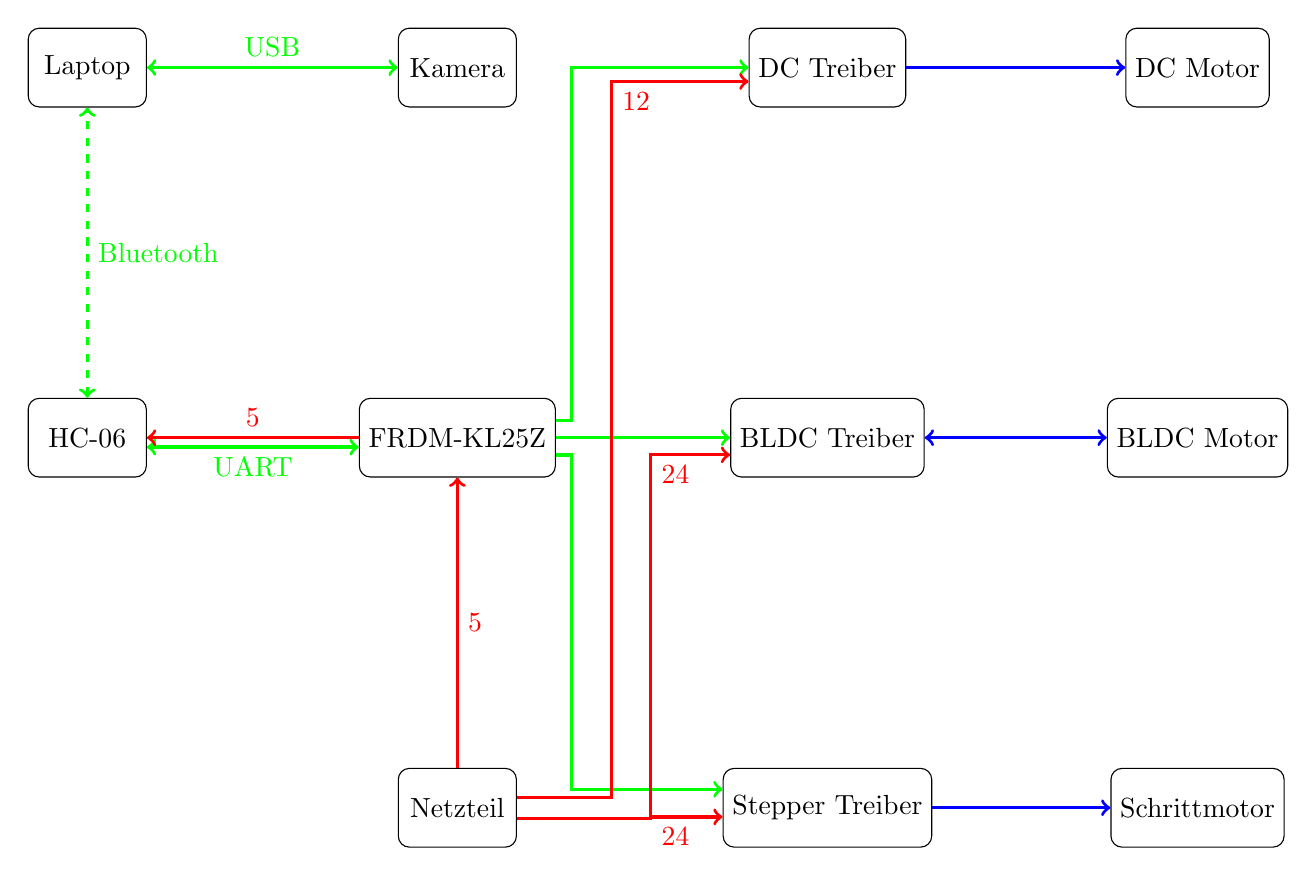
\begin{tikzpicture}[node distance=4.7cm]
        \node (frdm)        [block]                     {FRDM-KL25Z};
        \node (bt)          [block, left  of=frdm]      {HC-06};
        \node (computer)    [block, above of=bt]        {Laptop};
        \node (camera)      [block, right of=computer]  {Kamera};
        \node (supply)      [block, below of=frdm]      {Netzteil};
        \node (bldc-drv)    [block, right of=frdm]      {BLDC Treiber};
        \node (bldc)        [block, right of=bldc-drv]  {BLDC Motor};
        \node (step-drv)    [block, below of=bldc-drv]  {Stepper Treiber};
        \node (step)        [block, right of=step-drv]  {Schrittmotor};
        \node (dc-drv)      [block, above of=bldc-drv]  {DC Treiber};
        \node (dc)          [block, right of=dc-drv]    {DC Motor};
        % Data connections
        \draw[very thick, ->, green]    (frdm.350)          -| ++(0.2cm, 0)     |- (step-drv.170);
        \draw[very thick, ->, green]    (frdm.east)         -| ++(0.2cm, 0)     |- (bldc-drv.west);
        \draw[very thick, ->, green]    (frdm.10)           -| ++(0.2cm, 0)     |- (dc-drv.west);
        \draw[very thick, <->, green]   (frdm.base west)    -- node[below] {UART} (bt.base east);
        % Wireless data connection
        \draw[very thick, <->, green, dashed]   (bt)        -- node[right] {Bluetooth} (computer);
        \draw[very thick, <->, green]           (camera)    -- node[above] {USB} (computer);
        % Motor Power connections
        \draw[very thick, ->, blue]     (step-drv)  -- (step);
        \draw[very thick, <->, blue]    (bldc-drv)  -- (bldc);
        \draw[very thick, ->, blue]     (dc-drv)    -- (dc);
        % Power connections
        \draw[very thick, ->, red]  (frdm.west)      -- node[above] {5\si{\volt}}    (bt.east);
        \draw[very thick, ->, red]  (supply.north)   -- node[right] {5\si{\volt}}    (frdm);
        \draw[very thick, ->, red]  (supply.350)     -| ++(1.7cm, 0)     |- node[below right] {24\si{\volt}} (step-drv.185);
        \draw[very thick, ->, red]  (supply.350)     -| ++(1.7cm, 0)     |- node[below right] {24\si{\volt}} (bldc-drv.190);
        \draw[very thick, ->, red]  (supply.10)      -| ++(1.2cm, 0)     |- node[below right] {12\si{\volt}} (dc-drv.190);
    \end{tikzpicture}
    \caption{Übersicht Elektrotechnik}
\end{figure}
